\input{configuration}

\title{Lecture 12 --- Storage and Block Structure }

\author{Jeff Zarnett \\ \small \texttt{jzarnett@uwaterloo.ca}}
\institute{Department of Electrical and Computer Engineering \\
  University of Waterloo}
\date{\today}


\begin{document}

\begin{frame}
  \titlepage

 \end{frame}



\begin{frame}
\frametitle{Physical Storage}

Until this point in the course we have looked at databases more from the perspective of application developers.

This conceptual level has been useful for telling us about how to interact with databases and even how to (re)design data storage. 

That may have been entirely review for those who have significant experience with using databases. 

 \end{frame}



\begin{frame}
\frametitle{Physical Storage}


Now it is time to move into the implementation side of the database. 

\begin{center}
	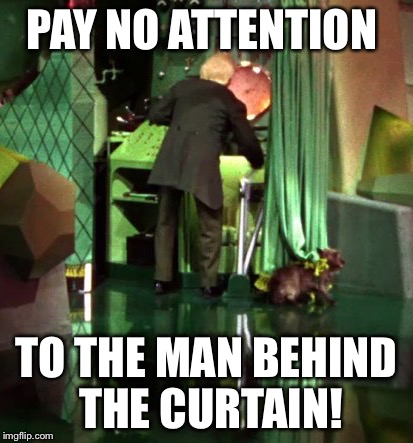
\includegraphics[width=0.4\textwidth]{images/curtain.jpg}
\end{center}

\end{frame}



\begin{frame}
\frametitle{How Data is Stored}

The fastest form of memory is registers, storage locations within the CPU itself. 

Then there is cache (often several levels of it), main memory, and finally, stable storage (solid state devices, magnetic hard drives, optical storage, and tapes). 

\end{frame}



\begin{frame}
\frametitle{Moving Data Around}

To actually do any of the operations we want to do in a reasonable time, the data must be moved from secondary storage to primary storage. 

Eventually if the data is to be saved/updated it has to be written back to secondary storage.

\end{frame}



\begin{frame}
\frametitle{Moving Data Around}

Secondary storage is generally very slow compared to primary storage. 

\begin{center}
	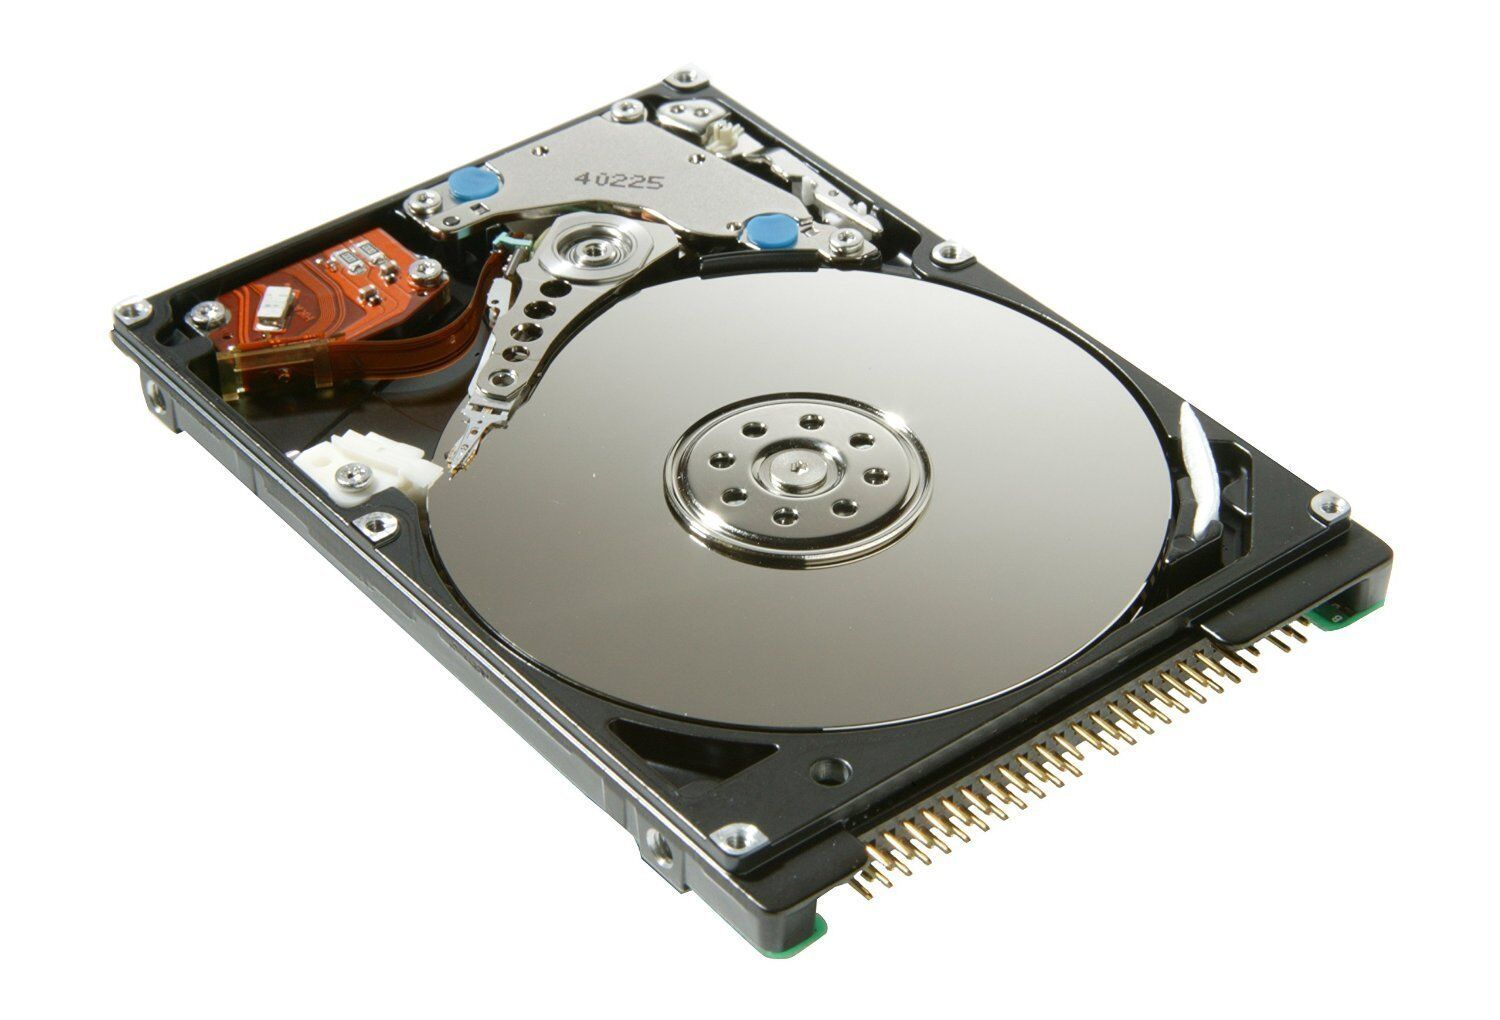
\includegraphics[width=0.45\textwidth]{images/hdd.jpg}
\end{center}

How we store our data becomes important because it determines how many times we need to access the slow storage...

And how much time we spend waiting for it.

\end{frame}



\begin{frame}
\frametitle{Over at the Temple / They Really Pack 'em in}

It's not as simple, unfortunately, as just packing as much into a block of storage as possible. 

We will still want to do that (usually) but there is more to it than just getting six records into a space where five used to fit. 

What is perhaps more important is: which five (or six) records to put in this particular block?


\end{frame}



\begin{frame}
\frametitle{Skip!}

Do we have to do this? Well, yes. 

(1) databases are too big for main memory (usually); 

(2) power outages and crashes DO happen, so nonvolatile storage is necessary; 

(3) secondary storage is affordable.


\end{frame}


\begin{frame}
\frametitle{Actually Storing Data}

Data is stored in files, and files correspond to blocks on disk. 

The \alert{primary file organization} determines how the file records are physically placed on disk (in the file, in the blocks). 

This obviously determines how we can access them. This is part of what determining the primary key is about. 

\end{frame}


\begin{frame}
\frametitle{Ordering}

Tuples of a relation as returned by a select query do not have a guaranteed ordering (unless there is an order-by clause). 

That is because they could be stored in a primary organization in multiple ways. 

\end{frame}


\begin{frame}
\frametitle{Ordering}
Our options could be:

\begin{enumerate}
	\item \textbf{Heap File}
	\item \textbf{Sorted File}
	\item \textbf{Hashed File}
	\item \textbf{B-Tree File}
\end{enumerate}

Extra work may be needed to sort!

\end{frame}



\begin{frame}
\frametitle{Secondary Organization}

A \alert{secondary organization} allows access to the data based on other criteria. 

An index is an example of a secondary organization which allows us to efficiently access the data based on that criterion. 

If we establish an index on an attribute, such as province in an address, it allows us to efficiently find tuples matching a particular province (e.g., ``SK'').

In the absence of that index, to find all addresses matching that province, we might have to scan all tuples.

\end{frame}


\begin{frame}
\frametitle{Placing Records on Disk}

The database will store records (tuples, relations, metadata, etc) on disk in a file or multiple files, as one would expect. 

The file itself is partitioned into blocks that match up with the file system's underlying architecture. 

Blocks are typically 4~KB but size may vary. 

Records are of variable size because they are user defined: if a user defines a relation with six attributes, a tuple in that relation may be a record.

\end{frame}



\begin{frame}
\frametitle{Fixed Length}

Let us imagine that a relation consists entirely of fixed length fields, so we can say that a tuple has a known size. 

If the sum of the fields' storage needs is, for example, 94 bytes, then we can fit 4096/94 = 43.57 records inside a block. 

\end{frame}



\begin{frame}
\frametitle{Fixed Length}


For performance reasons as well as to keep chaos down we will usually not allow a record to be split across two blocks. 

Thus we would round down and say that 43 records can fit in this block.

\end{frame}



\begin{frame}
\frametitle{Non-Fixed Length}

This assumes the relation consists entirely of fixed length fields. 

That is, sadly, not a safe assumption.

\begin{center}
	
\includegraphics[width=0.5\textwidth]{images/willem.jpg}
\end{center}

\end{frame}



\begin{frame}
\frametitle{Non-Fixed Length}


Variable length-records that fit within a single block are the subject for another series of allocation algorithms. 

Finally, if there is so much data that we cannot possibly fit it into a block, we will likely store the content elsewhere and just keep a pointer to it in the record.


\end{frame}



\begin{frame}
\frametitle{Fixed Length}

Assume for the moment that an individual file contains only one kind of record. 

If a record is of fixed length, then we can easily compute how long it will be in storage by simply summing up the length of the fields. 

A type ``instructor'' with attributes ID (varchar of 5), name (varchar 20), dept\_name (varchar 20), and salary (numeric 8,2).

That's easy enough to sum up if each character is assumed to be 1 byte and numeric 8,2 can be represented in 8 bytes.

\end{frame}



\begin{frame}
\frametitle{Fixed Length}
So the first 53 bytes are the first record, then the next 53 bytes are the second, and so on and so on and so on. 

77.28 records would fit in a 4K block and we round down meaning 77 records fit in an individual block. 

The rest of the space is wasted, in some sense, in the same way that we may have internal fragmentation in memory allocation requests.

\end{frame}



\begin{frame}
\frametitle{Spanned Records}

If we choose to allow a record to be in two blocks it is called \alert{spanned}:

\begin{center}
\includegraphics[width=0.7\textwidth]{images/spanned-unspanned}
\end{center}

In any case it is undesirable to have the record split even if it can be split cleanly because it doubles the amount of work to read or write this record.

A second problem is that it is difficult to delete a record in this structure.

\end{frame}



\begin{frame}
\frametitle{Performing Deletion}

\begin{center}
\includegraphics[width=0.4\textwidth]{images/instructor-1}
\end{center}



\begin{center}
\includegraphics[width=0.4\textwidth]{images/instructor-2} 
~~~~~~~~~~
\includegraphics[width=0.4\textwidth]{images/instructor-3}
\end{center}

\end{frame}



\begin{frame}
\frametitle{Fixed vs Variable Length}

Of course, things get complicated when we want to insert or delete records that are not fixed length. 

If we deleted record 3 in the previous example, what do we do if record 11 is bigger than record 3 was? Smaller? 

We clearly need a different strategy for variable length records.


\end{frame}


\begin{frame}
\frametitle{Variable Length Records}

If one field is of variable length then we have variable-length records in our file. 

\begin{center}
	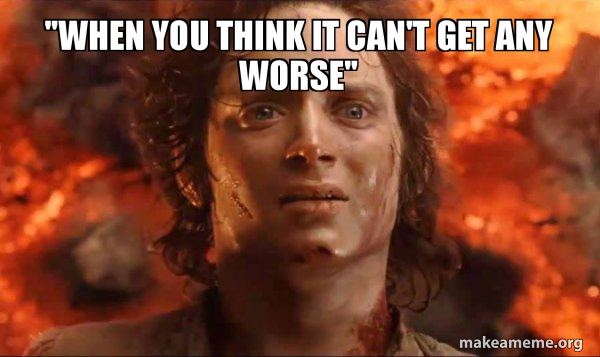
\includegraphics[width=0.4\textwidth]{images/frodo.jpg}
\end{center}

There are some other situations that might cause record length to vary.\\
\quad Repeating fields, optional fields, or multiple types of record in the same file. 

\end{frame}


\begin{frame}
\frametitle{Variable Length Records}

However the variable-length records are implemented, there are two operations we need to consider: 

(1) how to get records out of a block and\\ (2) how to get particular attributes from a record.

\end{frame}


\begin{frame}
\frametitle{Variable Length Records}

Variable length attributes are often represented in one of two ways. 

The first is a terminator character of some sort, something not normally allowed in the domain. 

The next is the attribute is prefixed with its length. 

\end{frame}


\begin{frame}
\frametitle{Variable Length Records}

\begin{center}
	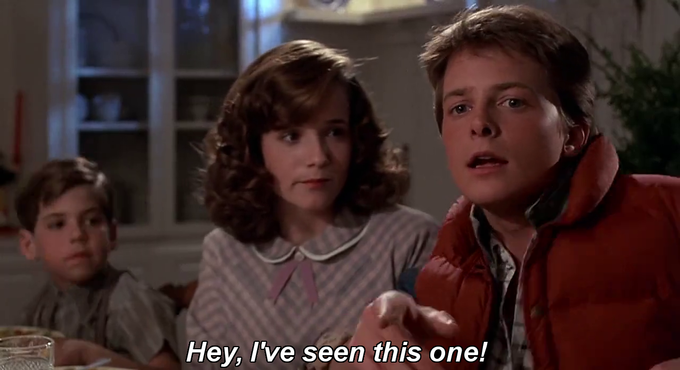
\includegraphics[width=0.4\textwidth]{images/seenthisone.png}
\end{center}

If these options sound familiar, they should, because they are the same ways programming languages might represent a variable length string.


\end{frame}


\begin{frame}
\frametitle{Variable Length Records}

The sample layout structure from suggests that fixed length attributes are put together. 

Then each variable length record has an entry of \textit{(offset, length)}  to explain where the variable length attribute is in the file. 

For the variable length record, if offset and attribute are 2 bytes each, then we have 4 bytes ``overhead'' per variable length attribute:

\begin{center}
\includegraphics[width=0.7\textwidth]{images/variable-length-record}
\end{center}

\end{frame}


\begin{frame}
\frametitle{Putting Variable Length Records in Blocks}
Then how do we put the variable length records into a block? 

For that, the strategy is the \alert{slotted page structure}.

The header includes the number of records in that block, where free space ends, and then an array with the location and size of each record.

\begin{center}
\includegraphics[width=0.7\textwidth]{images/slotted-page}
\end{center}

\end{frame}


\begin{frame}
\frametitle{Variable Length Records}

Records themselves are contiguous in the block and free space exists, perhaps counter-intuitively, between the end of the array and the first record.

If an entry is deleted the data is removed and any records between that record and the free space area are moved so that all free space remains contiguous.

If a record needs to grow or shrink due to an update statement, then we have to repeat the same procedures.

Reorganization following deletion does not have to take place immediately.

\end{frame}



\begin{frame}
\frametitle{Performance Considerations}

We can see that there are performance implications for whatever implementation strategy we choose. 

It's not our primary consideration, but is worth thinking about.

A select statement can take longer for certain requests than others...


\end{frame}




\end{document}

